\section{\METHOD~Network Architecture}
\label{section:method}

\begin{figure*}[t]
    \centering
    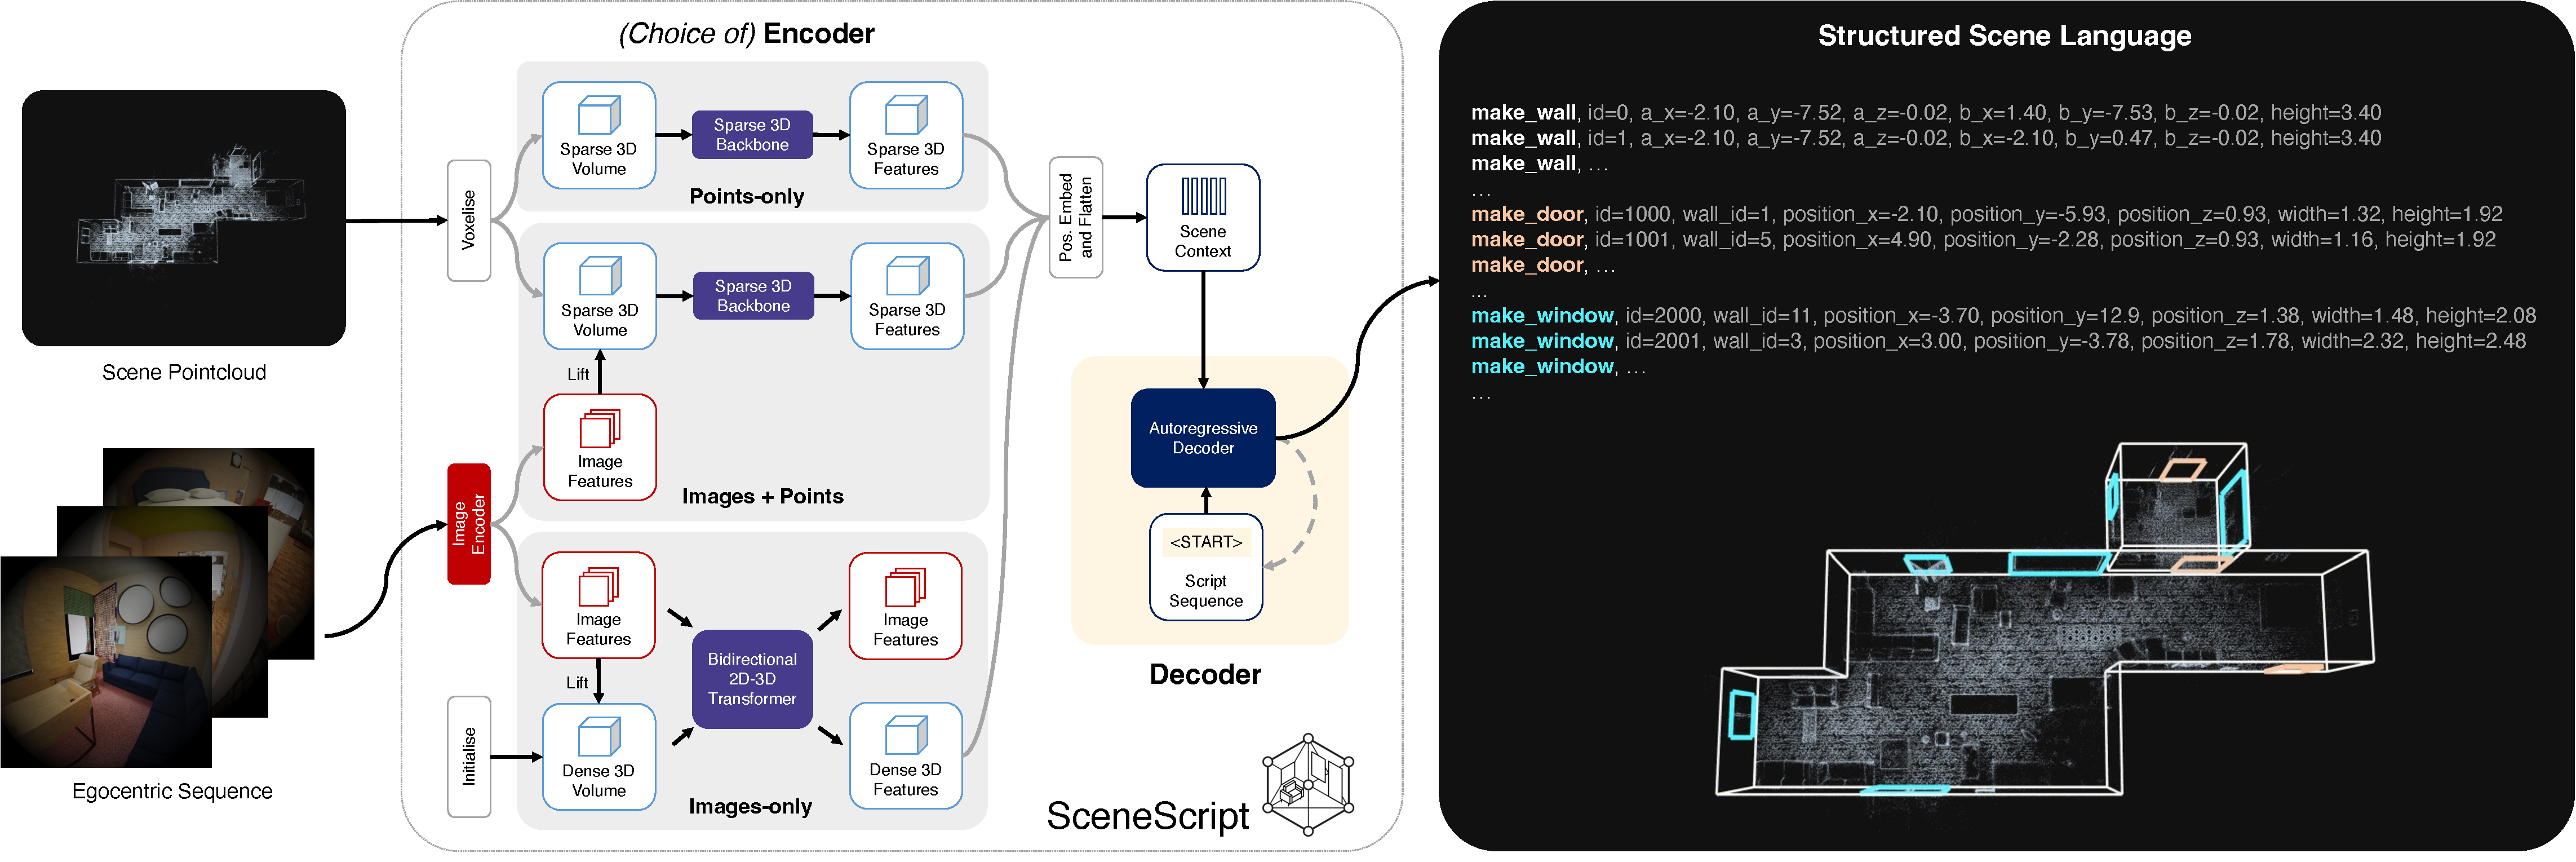
\includegraphics[width=\textwidth]{figs/alt_method_fig.pdf}\\[-3mm]
    % 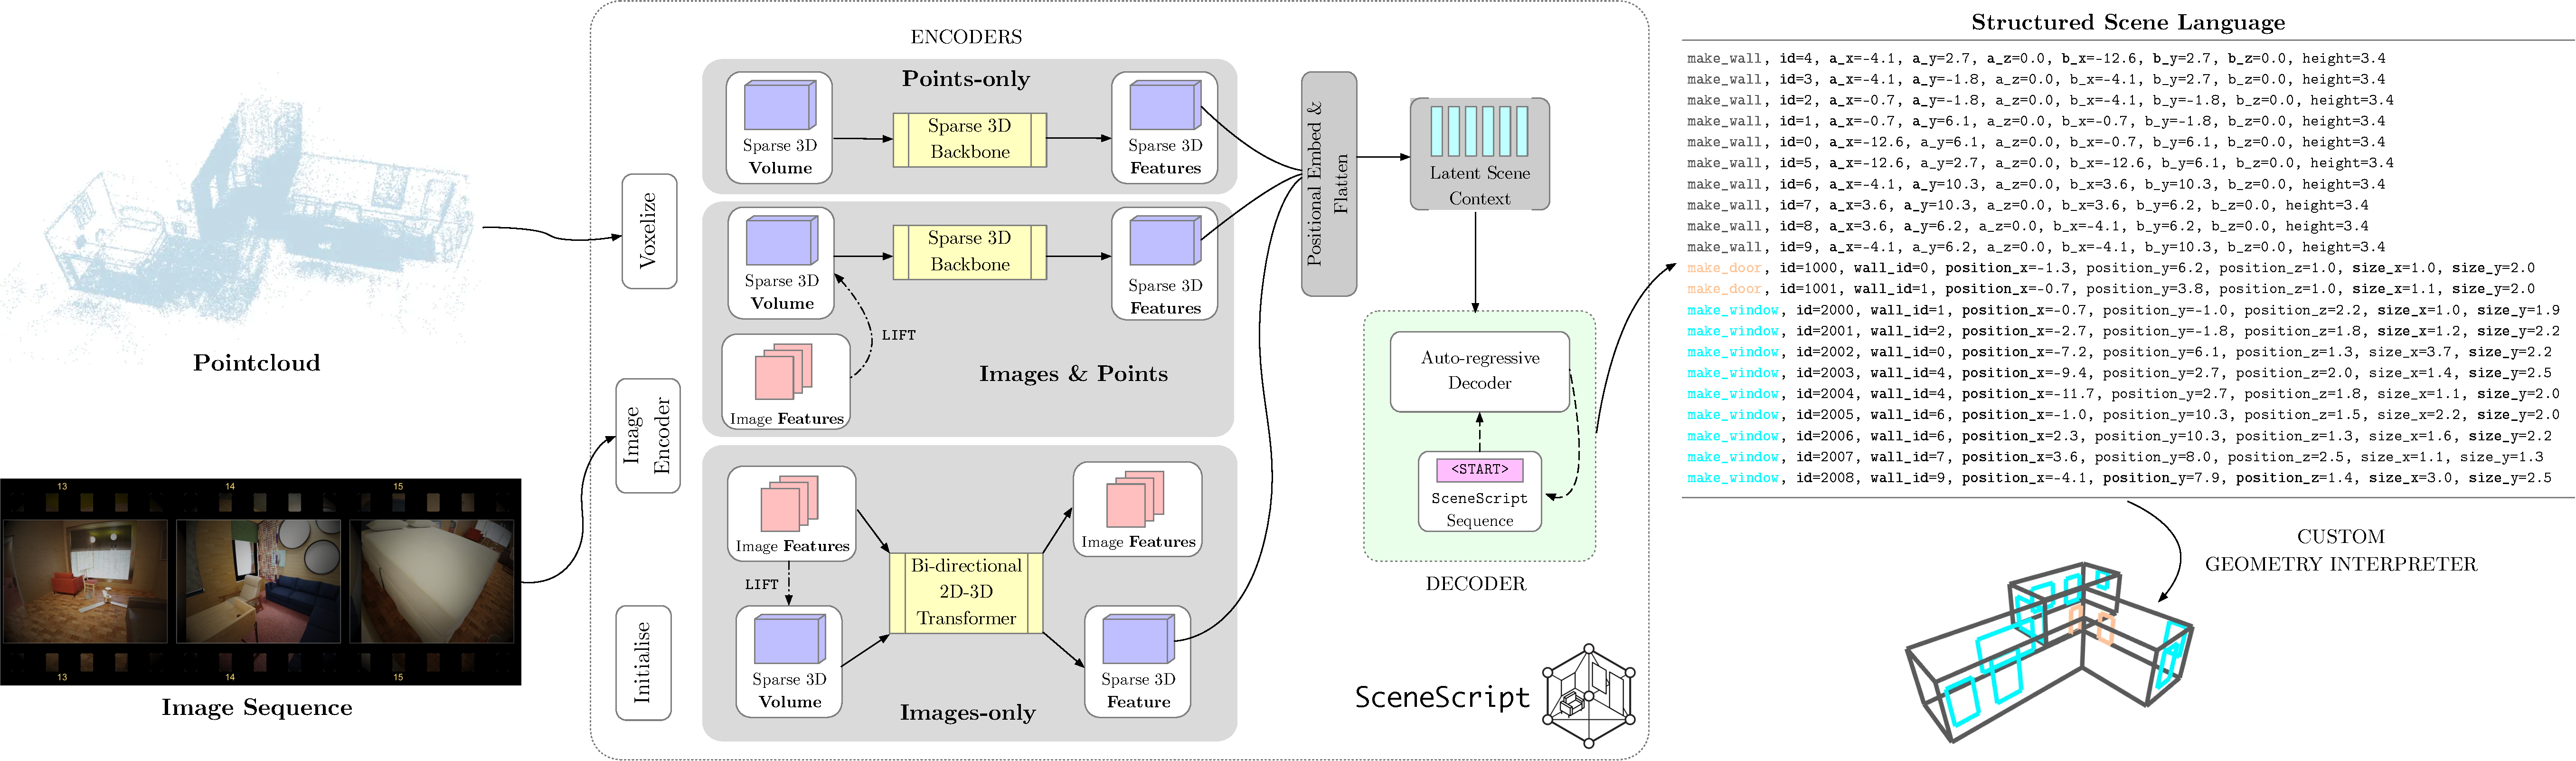
\includegraphics[width=\textwidth]{figs/Main-Figure.pdf}\\[-3mm]
    \caption{\METHOD~core pipeline overview. Raw images \& pointcloud data are encoded into a latent code, which is then autoregressively decoded into a sequence of commands that describe the scene. 
    Visualizations are shown using a customly built interpreter. Note that for the results in this paper, the the point clouds are computed from the images using Aria MPS \cite{aria_white_paper} -- i.e. are not using a dedicated RGB-D / Lidar sensor.}
    \label{fig:main_pipeline}
\end{figure*}

Our pipeline is a simple encoder-decoder architecture that consumes a video sequence and returns \METHOD~language in a tokenized format. Figure~\ref{fig:main_pipeline} illustrates a high-level overview of our method.

We examine three encoder variants: a pointcloud encoder, a posed image set encoder, and a combined encoder. The decoder remains the same in all cases.  


\subsection{Input Modalities and Encoders}
\label{sec:encoders}
%
The encoder computes a latent scene code
in the form of a 1D sequence
from video walkthrough of the scene.
The decoder is designed
to consume these 1D sequences as input.
This enables the integration of various input modalities
within a unified framework.
As a preliminary,
for each scene we assume access to
a set of $M$ posed camera images
$\{\mathbf{I_1},...,\mathbf{I_M}\}$, 
e.g., \SLAM{} output. 

\subsubsection{Point Clouds.}
\label{sec:encoder-points-only}

A point cloud 
$\mathbf{P} = \{\mathbf{p_1}, ..., \mathbf{p_N}\}$
consists of $N$ points,
where $\mathbf{p_i}$ is a 3D point coordinate. It can come from passive images using \SLAM{} or \SfM{}, or RGB-D / Lidar sensors.

Specifically, we use the Semi-dense Pointclouds from Project Aria's Machine Perception Services~\cite{aria_white_paper},
that are obtained from a visual-inertial SLAM system using Aria's monochrome cameras and IMUs. We discretize the point cloud to 5cm resolution, then employ a sparse 3D convolution library~\cite{tang2022torchsparse,tang2020searching} to generate pooled features. The encoder $\mathcal{E}_{geo}$ applies a series of down convolutions, resulting in a reduction of the number of points in the lowest level. 

\begin{equation}
\mathbf{F}_{geo} = \mathcal{E}_{geo}(\mathbf{P}), \quad \mathbf{P} \in \mathbb{R}^{N \times 3}, \mathbf{F}_{geo} \in \mathbb{R}^{K \times 512}
\end{equation}
where $K \ll N$. $\mathbf{F}_{geo}$ is a condensed latent representation of the point cloud that contains the necessary scene context. For later use in the transformer decoder, we treat $\mathbf{F}_{geo}$ as a sequence of feature vectors where the entries $\mathbf{f_i},\; i \in {1 ... K}$ are sorted lexicographically according to the coordinate of the active site $\mathbf{c_i},\; i \in {1 ... K}$. To incorporate positional encoding, we append the coordinates of the active sites to their respective feature vectors $\mathbf{f}_i \leftarrow \texttt{cat}(\mathbf{f_i}, \mathbf{c_i})$. 






\subsubsection{Point Clouds with Lifted Features.}

We additionally explore augmenting the point cloud with image features. From the original egocentric sequence and associated trajectory, we sample a set of $M$ keyframes, $\mathbf{I}_i$ where $i \in {1 ... M}$, and compute a set of image features $\mathbf{F}_i$ for each. We then project each point into the set of keyframe cameras and retrieve the feature vector (output by a CNN) at the pixel location:
\begin{equation}
    \mathbf{f}_{ip} = F_i(\pi(\mathbf{p})) \qquad \mathbf{p}\in\mathbf{P}, i \in {1 ... M},
\end{equation}
where $\pi(\cdot)$ represents the projection function of a 3D point into the camera. If $\pi(\mathbf{p})$ falls outside the image bounds, no feature is retrieved. We combine the set of lifted features for a point through an average, resulting in a single feature vector for each point: 
$\mathbf{f}_p = 1/M\sum_{i=1}^{M}{\mathbf{f}_{ip}}$.

We form our lifted-feature point cloud, $\mathbf{P'} = \{\mathbf{p'_1}, ..., \mathbf{p'_M}\}$, by  concatenating each point's lifted feature with the original XYZ location: $\mathbf{p}' = \texttt{cat}(\mathbf{f}_p,\mathbf{p})$. $\mathbf{P'}$ is then encoded into a context sequence using sparse 3D convolutions, with only the input feature channels adjusted to match the new point feature dimension.

\subsubsection{End-to-end Encoding of Posed Views.}
In order to encode the egocentric sequence more directly without a pre-computed point cloud, we adopt a 2D~$\leftrightarrow$~3D bidirectional transformer encoder following the form defined in RayTran~\cite{tyszkiewicz2022raytran}. 

In this formulation, we initialize a volume representation of the scene as a dense voxel grid of features, $\mathbf{V}$, that coincides with the scene geometry. In turn, we sample a subset of $M$ keyframes, $\mathbf{I}_i$ where $i \in {1 ... M}$, from the full stream of posed images. And for each of these keyframes we compute image features from a CNN, $\mathbf{F}_i$. 
Repeated layers of bidirectional attention enable the image and voxel grid features to be refined iteratively in successive transformer blocks through the aggregation of view-point and global-scene information. As in RayTran~\cite{tyszkiewicz2022raytran}, the interaction between the two representations is guided by the image-formation process by leveraging known camera parameters and poses. Attention in these transformer blocks is restricted by patch-voxel ray intersections, where each image patch attends to the voxels it observes and each voxel location attends to all the patches that observe it. The resulting voxel grid of features is flattened, concatenated with an encoded represention of its XYZ location, and passed to the decoder.







\subsection{Language Decoder}
\label{section:decoder}
%
We utilize a transformer decoder~\cite{vaswani2017attention} to decode the scene latent code into a sequence of structured language commands.
%, which is very effective in modelling long-range and functional relationships between parameter tokens of our modelling language. 
The sequence of tokens passes through an embedding layer, followed by a positional encoding layer. %to account for the ordering of the commands and parameters. 
Together with the encoded scene code (Section~\ref{sec:encoders}), the embedded tokens are passed into the several transformer decoder layers where a causal attention mask is used to ensure autoregressive generation. More implementation details can be found in 
Appendix~\ref{app:decoder}.
% the supplementary material.

\subsection{Language Tokenization}
\label{section:tokenization}
%
We refer to the serialization the structured language into a sequence of tokens as \textbf{tokenization}. The goal is to construct a bijective mapping between a sequence of structured language commands (Section~\ref{section:ssl}) and a sequence of integer tokens that can be predicted by the transformer decoder architecture. 
We utilize the following schema:
%
\begin{align*}
    &[ \paramstyle{col4}{START}, \paramstyle{col1}{PART}, \paramstyle{col2}{CMD},  \paramstyle{col2}{PARAM\_1},
    \paramstyle{col2}{PARAM\_2}, \ldots, \paramstyle{col2}{PARAM\_N}, \paramstyle{col1}{PART}, \ldots, \paramstyle{col4}{STOP} ] 
\end{align*}


For example, a sample sequence for a \texttt{make\_door} command may look like:
%
\begin{align*}
    &[ \paramstyle{col4}{START}, \paramstyle{col1}{PART}, \paramstyle{col2}{MAKE\_DOOR}, \paramstyle{col2}{POSITION\_X}, \paramstyle{col2}{POSITION\_Y}, \paramstyle{col2}{POSITION\_Z},\\
    &\paramstyle{col2}{WALL0\_IDX},  \paramstyle{col2}{WALL1\_IDX}, \paramstyle{col2}{WIDTH}, \paramstyle{col2}{HEIGHT},\paramstyle{col1}{PART}, \ldots, \paramstyle{col4}{STOP} ] 
\end{align*}
%
%The versatility and tolerance of this schema is evident because it 
This schema enables 1D packing of tokens without requiring fixed-size slots or padding like other sequence modelling methods such as \cite{wu2021deepcad}. Additionally, it does not impose any limitations on the number or the hierarchy of sub-sequences, as they are flexibly separated by a \paramstyle{col1}{PART} token. This allows for arbitrarily complex scene representations.

The tokenized sequence is discretized into integers at a 5cm resolution, then translated into a sequence of embeddings via learnable lookup table. Note that by designing the \METHOD~language, we also design the tokenization. This tokenization scheme is notably different from standard NLP tokenization, which involves Byte-Pair Encodings (BPE) \cite{openai2023gpt4}.



